\documentclass[tikz,border=3.14]{standalone}
\begin{document}

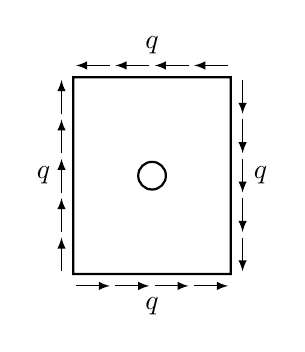
\begin{tikzpicture}[myarrow/.style={-latex,shorten >=1pt, shorten <=1pt}]
\draw[thick,nodes={outer sep=5pt}]
    circle[radius=5pt] 
    (-1,-1.25) 
    -- node[below] {$q$} ++(2,0)
    -- node[right] {$q$} ++(0,2.5)
    -- node[above] {$q$} ++(-2,0)
    -- node[left] {$q$} ++(0,-2.5)
    -- cycle
    ;
\foreach \i in {1,...,4}{
    \draw[myarrow] ({+1.5-\i*0.5},+1.4) -- ++(-.5,0);
    \draw[myarrow] ({-1.5+\i*0.5},-1.4) -- ++(+.5,0);
}
\foreach \j in {1,...,5}{
    \draw[myarrow] (-1.15,{-1.75+\j*0.5}) -- ++(0,+.5);
    \draw[myarrow] (+1.15,{+1.75-\j*0.5}) -- ++(0,-.5);
}
\end{tikzpicture}

\end{document}